\documentclass[12pt,dvipdfmx]{beamer}
\usepackage{graphicx}
\DeclareGraphicsExtensions{.pdf}
\DeclareGraphicsExtensions{.eps}
\graphicspath{{out/tex/lsvg/}{out/tex/svg/}{out/pdf/svg/}}

\usepackage{listings}
\usepackage{fancybox}
\usepackage{hyperref}
\usepackage{color}

\newcommand{\plusequal}{\mbox{\tt\ += }}
\newcommand{\minusequal}{\mbox{\tt\ -= }}
\newcommand{\divequal}{\mbox{\tt\ /= }}
\newcommand{\plusplus}{\mbox{\tt\ ++ }}



%% OpenMP section numbers
\newcommand{\sectionompparallel}{2.5}
\newcommand{\sectionompdeterminenumthreads}{2.5.1}
\newcommand{\sectionompfor}{2.7.1}
\newcommand{\sectionompdataenv}{2.14}
\newcommand{\sectionompgetnumthreads}{3.2.2}
\newcommand{\sectionompgetmaxthreads}{3.2.3}
\newcommand{\sectionompgetthreadnum}{3.2.4}


%%%%%%%%%%%%%%%%%%%%%%%%%%%
%%% themes
%%%%%%%%%%%%%%%%%%%%%%%%%%%
%\usetheme{Szeged} 
\usetheme{Madrid}

%% no navigation bar
% default boxes Bergen Boadilla Madrid Pittsburgh Rochester
%% tree-like navigation bar
% Antibes JuanLesPins Montpellier
%% toc sidebar
% Berkeley PaloAlto Goettingen Marburg Hannover Berlin Ilmenau Dresden Darmstadt Frankfurt Singapore Szeged
%% Section and Subsection Tables
% Copenhagen Luebeck Malmoe Warsaw

%%%%%%%%%%%%%%%%%%%%%%%%%%%
%%% innerthemes
%%%%%%%%%%%%%%%%%%%%%%%%%%%
% \useinnertheme{circles}	% default circles rectangles rounded inmargin

%%%%%%%%%%%%%%%%%%%%%%%%%%%
%%% outerthemes
%%%%%%%%%%%%%%%%%%%%%%%%%%%
% outertheme
% \useoutertheme{default}	% default infolines miniframes smoothbars sidebar sprit shadow tree smoothtree


%%%%%%%%%%%%%%%%%%%%%%%%%%%
%%% colorthemes
%%%%%%%%%%%%%%%%%%%%%%%%%%%
\usecolortheme{seahorse}
%% special purpose
% default structure sidebartab 
%% complete 
% albatross beetle crane dove fly seagull 
%% inner
% lily orchid rose
%% outer
% whale seahorse dolphin

%%%%%%%%%%%%%%%%%%%%%%%%%%%
%%% fontthemes
%%%%%%%%%%%%%%%%%%%%%%%%%%%
\usefonttheme{serif}  
% default professionalfonts serif structurebold structureitalicserif structuresmallcapsserif

%%%%%%%%%%%%%%%%%%%%%%%%%%%
%%% generally useful beamer settings
%%%%%%%%%%%%%%%%%%%%%%%%%%%
% 
\AtBeginDvi{\special{pdf:tounicode EUC-UCS2}}
% do not show navigation
\setbeamertemplate{navigation symbols}{}
% show page numbers
\setbeamertemplate{footline}[frame number]


%%%%%%%%%%%%%%%%%%%%%%%%%%%
%%% define some colors for convenience
%%%%%%%%%%%%%%%%%%%%%%%%%%%

%\newcommand{\mido}[1]{{\color{green}#1}}
\newcommand{\mido}[1]{{\color{green}#1}}
\newcommand{\mura}[1]{{\color{purple}#1}}
\newcommand{\ore}[1]{{\color{orange}#1}}
\newcommand{\ao}[1]{{\color{blue}#1}}
\newcommand{\aka}[1]{{\color{red}#1}}

\setbeamercolor{ex}{bg=cyan!20!white}

%%%%%%%%%%%%%%%%%%%%%%%%%%%
%%% how to typset code
%%%%%%%%%%%%%%%%%%%%%%%%%%%

\lstset{language = C,
numbers = left,
numberstyle = {\tiny \emph},
numbersep = 10pt,
breaklines = true,
breakindent = 40pt,
frame = tlRB,
frameround = ffft,
framesep = 3pt,
rulesep = 1pt,
rulecolor = {\color{blue}},
rulesepcolor = {\color{blue}},
flexiblecolumns = true,
keepspaces = true,
basicstyle = \ttfamily\scriptsize,
identifierstyle = ,
commentstyle = \it\scriptsize,
stringstyle = ,
showstringspaces = false,
tabsize = 4,
escapechar=\@,
}

\title{Neural Networks Basics}
\institute{}
\author{Kenjiro Taura}
\date{}

\AtBeginSection[] % Do nothing for \section*
{
\begin{frame}
\frametitle{Contents}
\tableofcontents[currentsection]
\end{frame}
}

\AtBeginSubsection[] % Do nothing for \section*
{
\begin{frame}
\frametitle{Contents}
\tableofcontents[currentsection,currentsubsection]
\end{frame}
}

\begin{document}
\maketitle

%%%%%%%%%%%%%%%%%%%%%%%%%%%%%%%%%% 
\begin{frame}
\frametitle{Contents}
\tableofcontents
\end{frame}

\newcommand{\Convolution}{\mbox{Convolution}}
\newcommand{\Linear}{\mbox{Linear}}
\newcommand{\relu}{\mbox{relu}}
\newcommand{\ReLU}{\mbox{ReLU}}
\newcommand{\maxpool}{\mbox{maxpool}}
\newcommand{\relutwo}{\mbox{relu2}}
\newcommand{\ReLUtwo}{\mbox{ReLU2}}
\newcommand{\softmax}{\mbox{softmax}}
\newcommand{\logsoftmax}{\mbox{logsoftmax}}
\newcommand{\nll}{\mbox{NLL}}
\newcommand{\crossentropy}{\mbox{cross\_entropy}}
\newcommand{\pp}[2]{\frac{\partial #1}{\partial #2}}
\newcommand{\ppt}[2]{\frac{{}^t\partial #1}{\partial #2}}
\newcommand{\vecthree}[3]{\left(\begin{array}{c} #1 \\ #2 \\ #3 \end{array}\right)}
\newcommand{\mathree}[9]{\left(\begin{array}{ccc} #1 & #2 & #3 \\ #4 & #5 & #6 \\ #7 & #8 & #9 \end{array}\right)}
\newcommand{\sign}{\mbox{sign}}
\newcommand{\diag}{\mbox{diag}}

%%%%%%%%%%%%%%%%%
\section{What is machine learning?}
%%%%%%%%%%%%%%%%% 

%%%%%%%%%%%%%%%%% 
\begin{frame}
\frametitle{What is machine learning?}
\begin{itemize}
\item<1-> \ao{input:} a set of \ao{\emph{training data set}}
\[ D = \{\;(x_i,t_i)\;|\; i = 0, 1, \cdots \;\} \]

\begin{itemize}
\item<1-> each \ao{$x_i$} is normally a real vector (i.e. many real values)
\item<1-> each \ao{$t_i$} is a real value (regression), 
  0/1 (binary classification),
  a discrete value (multi-class classification), 
  etc., depending on the task
\end{itemize}

\item<2-> \ao{goal:} a supervised machine learning tries 
to find a function $f$ that ``matches'' training data well. i.e.
\[ f(x_i) \approx t_i \mbox{ for } (x_i,t_i) \in D \]

\item<2-> put formally, find $f$ that minimizes 
  an \emph{error} or a \emph{loss}:
\[ \ao{L(f; D) \equiv \sum_{(x_i,t_i)\in D} \mbox{err}(f(x_i), t_i),} \]
where \ao{$\mbox{err}(y_i, t_i)$} is a function that measures
an ``error'' or a  ``distance'' 
between the predicted output and the true value
\end{itemize}
\end{frame}

%%%%%%%%%%%%%%%%% 
\begin{frame}
\frametitle{Machine learning as an optimization problem}
\begin{itemize}
\item<1-> finding a good function from 
  the space of {\it literally all} possible functions is neither easy nor meaningful

\item<1-> we thus normally fix a search space of functions (${\cal{F}}$)
  to a fixed expression parameterized by $w$ 
  and find a good function $f_w \in {\cal{F}}$ \ao{\emph{(parametric models)}}

\item<2-> the task is then to find the value of $w$ 
  that minimizes the loss:
\[ L(\ao{w}; D) \equiv \sum_{(x_i,t_i)\in D} \mbox{err}(\ao{f_w}(x_i), t_i) \]
\end{itemize}
\end{frame}

%%%%%%%%%%%%%%%%% 
\subsection{A simple linear regression}
%%%%%%%%%%%%%%%%% 

%%%%%%%%%%%%%%%%% 
\begin{frame}
\frametitle{A simple example (linear regression)}
\begin{itemize}
\item<1-> training data $D = \{\; (x_i,t_i)\;|\; i = 0, 1, \cdots \}$
  \begin{itemize}
  \item $x_i$ : a real value
  \item $t_i$ : a real value
  \end{itemize}

\item<2-> let the search space be a set of polynomials of degree $\leq 2$.
  a function is then parameterized by $\ao{w = (w_0\;w_1\;w_2)}.$ i.e.
  \[ f_{\ao{w}}(x) \equiv \ao{w_2} x^2 + \ao{w_1} x + \ao{w_0} \]

\item<3-> let the error function be a simple square distance:
  \[ \mbox{err}(y, t) \equiv (y - t)^2 \]

\item<4-> the task is to find $w = (w_0, w_1, w_2)$ that minimizes:
  \[ L(\ao{w}; D) = \sum_{(x_i,t_i)\in D} 
  \mbox{err}(f_w(x_i),t_i) 
= \sum_{(x_i,t_i)\in D} (\ao{w_2} x_i^2 + \ao{w_1} x_i + \ao{w_0} - t_i)^2 \]
\end{itemize}
\end{frame}

%%%%%%%%%%%%%%%%% 
\subsection{A handwritten digit recognition}
%%%%%%%%%%%%%%%%% 

%%%%%%%%%%%%%%%%% 
\begin{frame}
\frametitle{A more realistic example: digit recognition}
\begin{columns}
\begin{column}{0.75\textwidth}
\begin{itemize}
\item<1-> training data $D = \{\;(x_i,t_i)\;|\; i = 0, 1, \cdots \}$
  \begin{itemize}
  \item $x_i$ : a vector of pixel values of an image:
  \item $t_i$ : the class of $x_i$ ($t_i \in \{ 0, 1, \cdots , 9 \}$)
    % (e.g. $\sim {}^t(0\;0\;0\;0\;1\;0\;0\;0\;0\;0\;0)$ represents ``4'')
  % \item we write \textbf{i} to mean the hot vector $v$ having $v_i = 1$
  %   \begin{center}
  %     $D = \{
  %     (
\includegraphics[width=0.6cm]{out/pdf/img/mnist_four.pdf}, \textbf{4}),
  %     (
\includegraphics[width=0.6cm]{out/pdf/img/mnist_nine.pdf}, \textbf{9}), \ldots \}$
  %   \end{center}
  \end{itemize}

\item<2-> the search space: the following composition
  parameterized by three matrices \ao{$W_0$}and {$W_1$}
\[ f_{\ao{W_0,W_1}} (x) \equiv \softmax(\ao{W_1} \maxpool(\ReLU(\ao{W_0} \ast x))) \]

\end{itemize}
\end{column}

\begin{column}{0.25\textwidth}
\begin{center}
\only<2->{\def\svgwidth{0.7\textwidth}%
{\tiny\input{out/tex/svg/mnist_pytorch_1.pdf_tex}}}
\end{center}
\end{column}
\end{columns}
\end{frame}


%%%%%%%%%%%%%%%%% 
\begin{frame}
\frametitle{A handwritten digits recognition}
\begin{columns}
\begin{column}{0.75\textwidth}
\begin{itemize}
\item<1-> the output $y = f_{W_0,W_1}(x)$
  is a 10-vector representing probabilities that $x$ belongs to each of the ten classes

% \item<2-> a loss function is the cross entropy commonly used in multiclass classifications ($\cdot$ : a dot product)
% \[ \mbox{err}(y, t) = H(t, y) \equiv - t \cdot \log y \]

\item<2-> a loss function is {\it negative log-likelihood}
  commonly used in multiclass classifications
  \[ \mbox{err}(y, t) = \nll(y, t) \equiv - \log y_t \]

\item<3> the task is to find $W_0$ and $W_1$ that minimize:
  {\scriptsize
  \begin{eqnarray*}
    &  & L(\ao{W_0, W_1}; D) \\
    & = & \sum_{(x_i,t_i)\in D} \nll(f_{W_0,W_1}(x_i), t_i) \\
    & = & \sum_{(x_i,t_i)\in D}
          \nll(\softmax(\ao{W_1} \maxpool(\ReLU(\ao{W_0} \ast x))), t_i)
  \end{eqnarray*}}
\end{itemize}
\end{column}

\begin{column}{0.25\textwidth}
\begin{center}
\def\svgwidth{0.7\textwidth}
{\tiny\input{out/tex/svg/mnist_pytorch_2.pdf_tex}}
\end{center}
\end{column}
\end{columns}
\end{frame}

%%%%%%%%%%%%%%%%% 
\section{Training}
%%%%%%%%%%%%%%%%% 

%%%%%%%%%%%%%%%%% 
\subsection{A simple gradient descent}
%%%%%%%%%%%%%%%%% 

%%%%%%%%%%%%%%%%% 
\begin{frame}
\frametitle{How to find the minimizing parameter?}
\begin{itemize}
\item it boils down to minimizing a function that takes 
  \emph{lots of} parameters $w$
\[ L(\ao{w}; D) = \sum_{(x_i,t_i)\in D} \mbox{err}(f_{\ao{w}}(x_i), t_i), \]

\item we compute \ao{the derivative
  of $L$ with respect to $w$} and move $w$ to its opposite
  direction \ao{\emph{(gradient descent; GD)}}

\[ \ao{w = w - \eta {}^t \pp{L}{w}} \]
($\eta$ : a small value controlling a learning rate)

\item repeat this until $L(w; D)$ converges
\end{itemize}
\end{frame}

%%%%%%%%%%%%%%%%% 
\begin{frame}
\frametitle{Why GD works}
\begin{itemize}
\item recall
  \[ L(w + \Delta w; D) \approx L(w; D) + \pp{L}{w} \Delta w \]
  
\item so, by moving $w$ slightly to the direction of gradient (i.e., $\Delta w = - \eta\ppt{L}{w}$ for small $\eta$),

  \begin{eqnarray*}
    L(w - \eta \ppt{L}{w}; D) & \approx & L(w; D) -\eta \pp{L}{w} \ppt{L}{w} \\
                                 & < & L(w; D)
  \end{eqnarray*}
$L$ will decrease
\end{itemize}
\end{frame}


%%%%%%%%%%%%%%%%% 
\begin{frame}
\frametitle{A linear regression example}
\begin{itemize}
\item<1-> recall that in the linear regression example:
\[ L(w; D) = \sum_{(x_i,t_i)\in D} (w_2 x_i^2 + w_1 x_i + w_0 - t_i)^2 \]

\item<2-> differentiate $L$ by $w = {}^t(w_0\;\;w_1\;\;w_2)$ to get:
\[ \pp{L}{w} = \sum_{(x_i,t_i)\in D} 2 (w_2 x_i^2 + w_1 x_i + w_0 - t_i) (1\;\;x_i\;\;x_i^2) \]
(remark: we used \ao{a chain rule})

\item<3-> so you repeat:
 \[ w = w - \eta \sum_{(x_i,t_i)\in D} 2 (w_2 x_i^2 + w_1 x_i + w_0 - t_i) \vecthree{1}{x_i}{x_i^2} \]
until $L(w; D)$ converges
\end{itemize}
\end{frame}

%%%%%%%%%%%%%%%%% 
\begin{frame}
\frametitle{A problem of the gradient descent}
\begin{itemize}
\item<1-> the loss function we want to minimize is normally a summation over
  \ao{\emph{all}} training data:
\[ L(w; D) = \ao{\sum_{(x_i,t_i)\in D}} \mbox{err}(f_w(x_i), t_i) \]

\item<2-> the gradient descent method just described:
  \begin{enumerate}
  \item computes ${\displaystyle\pp{}{w}\mbox{err}(f_w(x_i), t_i)}$ for each training data $(x_i,t_i) \in D$,
    \ao{\emph{with the current value of $w$}}
  \item sum them over \ao{\emph{whole data set}} and then update $w$
  \end{enumerate}
  
\item<3-> it is commonly observed that the
  convergence becomes faster when we update
  $w$ more ``incrementally'' $\rightarrow$ 
  \ao{\emph{Stochastic Gradient Descent (SGD)}}
\end{itemize}
\end{frame}

%%%%%%%%%%%%%%%%% 
\subsection{Stochastic gradient descent}
%%%%%%%%%%%%%%%%% 

%%%%%%%%%%%%%%%%% 
\begin{frame}
\frametitle{SGD}

repeat:
\begin{enumerate}
\item<1-> randomly draw a \ao{\emph{subset}} of training data $D'$ (a mini batch; $D' \subset D$)
\item<2-> compute the gradient of loss \ao{\emph{over the mini batch}}
\[ \pp{L(w; \ao{D'})}{w} = \sum_{(x_i,t_i)\in \ao{D'}} \pp{}{w} \mbox{err}(f_w(x_i), t_i) \]
\item<3-> update $w$
\[ w = w - \eta {}^t \pp{L(w; \ao{D'})}{w} \]

\item<3-> ``update sooner rather than later''
\end{enumerate}
\end{frame}

%%%%%%%%%%%%%%%%% 
\begin{frame}
\frametitle{Computing the gradients}
\begin{columns}
\begin{column}{0.6\textwidth}
\begin{itemize}
\item in neural networks, a function is a composition of many stages
each represented by a lot of parameters
\begin{eqnarray*}
x_1 & = & f_1(\ao{w_1}; x) \\
x_2 & = & f_2(\ao{w_2}; x_1) \\
    & \ldots &  \\
 y  & = & f_n(\ao{w_n}; x_n) \\
 \ao{\ell}  & = & \mbox{err}(y, t)
\end{eqnarray*}
\item we need to differentiate \ao{$\ell$} by $w_1, \cdots, w_n$
\end{itemize}
  \end{column}
  
\begin{column}{0.4\textwidth}
\begin{center}
\def\svgwidth{\textwidth}
{\scriptsize\input{out/tex/svg/nn_stage.pdf_tex}}
\end{center}
\end{column}
\end{columns}
\end{frame}


%%%%%%%%%%%%%%%%% 
\begin{frame}
\frametitle{The digit recognition example}

\begin{columns}[t]
\begin{column}{0.7\textwidth}
  \begin{itemize}
  \item []
\begin{eqnarray*}
x_1 & = & \ao{W_0} \ast x \\
x_2 & = & \ReLU(x_1) \\
x_3 & = & \maxpool(x_2) \\
x_4 & = & \ao{W_1}x_3 \\
  y & = & \softmax(x_4) \\
\ao{\ell} & = & \nll(y, t)
\end{eqnarray*}
\item [] you need to differentiate \ao{$\ell$}
  by \ao{$W_0$} and \ao{$W_1$}
\end{itemize}
\end{column}

\begin{column}{0.25\textwidth}
\begin{center}
\def\svgwidth{0.7\textwidth}
{\tiny\input{out/tex/svg/mnist_pytorch_2.pdf_tex}}
\end{center}
\end{column}
\end{columns}
\end{frame}

%%%%%%%%%%%%%%%%% 
\section{Chain Rule}
%%%%%%%%%%%%%%%%% 

\iffalse
%%%%%%%%%%%%%%%%% 
\begin{frame}
\frametitle{Derivative of multivariable functions}
\begin{itemize}
\item $x = {}^t(x_0\; \cdots\; x_{n-1}) \in R^n$ (a column vector)
\item $f(x) \in R$ (a scalar. presumably a loss function)

\item \ao{\textbf{definition:}}
  a derivative of $f$ with respect to $x$,
  written $f'(x)$, is a row vector $a$ s.t.

  \begin{eqnarray*}
    \Delta f & \equiv & f(x + \Delta x) \\
             & \approx & f(x) + a \Delta x \\
             & = & f(x) + \sum_i a_i \Delta x_i \\
  \end{eqnarray*}

\item when $f'(x)$ exists, it is

  \[ f'(x) = \left(\pp{f}{x_0} \; \cdots \; \pp{f}{x_{n-1}}\right) \]
  
\item a partial derivative $\pp{f}{x_i}$ is a scalar $a_i$ s.t.
  
  \[ f'(x_0, \cdots , x_i + \Delta x_i , \cdots , x_{n-1}) =
    f(x) + a_i \Delta x_i \]
\end{itemize}
\end{frame}
\fi

%%%%%%%%%%%%%%%%% 
\begin{frame}
\frametitle{Differentiating multivariable functions}
\begin{itemize}
\item $x = {}^t(x_0 \; \cdots\; x_{n-1}) \in R^n$ (a column vector)
\item $f(x)$ : a scalar

\item \ao{\textbf{definition:}}
  the gradient of $f$ with respect to $x$, 
  written ${\displaystyle \pp{f}{x}}$,
  is \ao{a row $n$-vector} s.t.
  {\footnotesize
  \begin{eqnarray*}
    \Delta f & \equiv & f(x + \Delta x) - f(x) \\
             & \approx & \pp{f}{x} \Delta x \\
             & = & \sum_{i=0}^{n-1} \left(\pp{f}{x}\right)_i \Delta x_i
  \end{eqnarray*}}
%(a row vector $\times$ a column vector, yielding
%a $1\times 1$ matrix, identified with a scalar)

\item when it exists, 
  {\footnotesize \[ \pp{f}{x} = \left(\pp{f}{x_0}\;\cdots\;\pp{f}{x_{n-1}}\right), \]}
  so
  \ao{\footnotesize\[ \Delta f \approx \sum_{i=0}^{n-1} \pp{f}{x_i} \Delta x_i \]}
\end{itemize}
\end{frame}


%%%%%%%%%%%%%%%%% 
\begin{frame}
\frametitle{The Chain Rule}
\begin{itemize}
\item consider a function $f$ that depends on
  $y = (y_0, \cdots , y_{m-1}) \in R^{m}$,
  each of which in turn depends on $x = (x_0, \cdots , x_{n-1}) \in R^n$

\item \ao{the chain rule (math textbook version):}

  \[ \pp{f}{x_i} = \sum_{0 \leq j < m} \pp{f}{y_j} \pp{y_j}{x_i}
    \quad (0 \leq i < n)
  \]

\begin{center}
\def\svgwidth{0.45\textwidth}
{\scriptsize\input{out/tex/svg/chain_intuition_1.pdf_tex}}
\end{center}

\end{itemize}
\end{frame}


%%%%%%%%%%%%%%%%% 
\begin{frame}
\frametitle{The Chain Rule : intuition}
\begin{center}
\def\svgwidth{0.4\textwidth}
{\scriptsize\input{out/tex/svg/chain_intuition_1.pdf_tex}}
\end{center}
\vskip-0.5cm
\begin{itemize}
\item say you increase an input variable $x_i$ by $\Delta x_i$, 
  each $y_j$ will increase by
  \[ \approx \pp{y_j}{x_i}\Delta x_i, \]
  which will contribute to increasing the final output ($f$) by
  \[ \approx \pp{f}{y_j} \pp{y_j}{x_i}\Delta x_i \]
\end{itemize}
\end{frame}


%%%%%%%%%%%%%%%%% 
\begin{frame}
\frametitle{Chain Rule}
\begin{itemize}
\item master the following ``index-free'' version for neural network
  
\item $x$, $y$ : a scalar
  (a single component in a vector/matrix/high dimensional array)

\item \ao{the chain rule (ML practioner's version):}
  
  \[ \ao{\pp{f}{x} = \sum_{\mbox{{\tiny all variables $y$ that $x$ {\it directly} affects}}}
    \pp{f}{y} \pp{y}{x}}
  \]

\begin{center}
\def\svgwidth{0.25\textwidth}
{\scriptsize\input{out/tex/svg/chain_intuition_2.pdf_tex}}
\end{center}

\end{itemize}
\end{frame}


%%%%%%%%%%%%%%%%% 
\begin{frame}
  \frametitle{Chain Rule and ``Back Propagation''}
  \begin{columns}
    \begin{column}{0.6\textwidth}
{\footnotesize      
\begin{itemize}
\item Chain rule allows you to compute
  \[ \pp{L}{x}, \]
  the derivative of the loss with respect to a variable,
  from
  \[ \pp{L}{y}, \]
  the derivatives of the loss with respect to upstream variables

  \[ \ao{\pp{L}{x}
      = \sum_{\mbox{{\tiny all variables $y$ a step ahead of $x$}}}
      \pp{L}{y} \pp{y}{x}}
  \]
\end{itemize}}
\end{column}
\begin{column}{0.4\textwidth}
\begin{center}
\def\svgwidth{0.45\textwidth}
{\tiny\input{out/tex/svg/mnist_pytorch_2.pdf_tex}}
\end{center}
\end{column}
\end{columns}
  

\end{frame}

\iffalse
%%%%%%%%%%%%%%%%% 
\subsection{Vector fields}
%%%%%%%%%%%%%%%%% 

%%%%%%%%%%%%%%%%% 
\begin{frame}
\frametitle{Differentiating multivariable functions (vector fields)}
\begin{itemize}
\item $f$ : a vector field
  \begin{itemize}
  \item $x \in R^n$ (column vector)
  \item $y = f(x) \in \ao{R^m}$ (column vector)
  \end{itemize}

\item \ao{\textbf{definition:}} a derivative of $f$ with respect to $x$, 
  written $f'(x)$ or ${\displaystyle \pp{f}{x}}$, is 
  \ao{a $m \times n$ matrix $A$} s.t.
\[ f(x + \Delta x) \approx f(x) + \ao{A} \; \Delta x \]

\item when it exists, 
\[ A = \left(\pp{y_i}{x_j}\right)_{i,j} \]

\end{itemize}
\end{frame}

\newcommand{\rin}{\rotatebox[origin=c]{-90}{$\in$}}

%%%%%%%%%%%%%%%%% 
\subsection{Chain Rule}
%%%%%%%%%%%%%%%%% 

%%%%%%%%%%%%%%%%% 
\begin{frame}
\frametitle{Chain rule}
\begin{itemize}
\item given these definitions, a familiar/beautiful 
chain rule applies for functions taking a vector as input
\begin{itemize}
\item $x \in R^n$
\item $y = f(x) \in R^m$
\item $z = g(y) \in R^l$
\end{itemize}
\item then we have:
\[
\begin{array}{rcll}
{\displaystyle\ao{\pp{z}{x}}}     & \ao{=} & {\displaystyle\ao{\pp{z}{y}}}     & {\displaystyle\ao{\pp{y}{x}}}   \\
 \rin            &        & \rin               & \rin          \\
R^{l\times n}      &        & R^{l\times m}       & R^{m\times n} \\
\end{array}
\]

\item remark: it holds for derivatives defined as matrices;
  individual partial derivatives do not enjoy such beautiful properties
\end{itemize}
\end{frame}

%%%%%%%%%%%%%%%%% 
\begin{frame}
\frametitle{Chain rule and neural network (1)}
\begin{columns}
\begin{column}{0.6\textwidth}
\begin{itemize}
\item chain rule:
\[ \pp{z}{x} = \pp{z}{y} \pp{y}{x} \]
gives a tool to compute a derivative of
the loss function with respect to any 
input/intermediate \ao{\emph{vectors}}


\end{itemize}
\end{column}

\begin{column}{0.4\textwidth}
\begin{center}
\def\svgheight{\textheight}
{\scriptsize\input{out/tex/svg/chain_1.pdf_tex}}
\end{center}
\end{column}  
\end{columns}
\end{frame}

%%%%%%%%%%%%%%%%% 
\begin{frame}
\frametitle{Chain rule and neural network (2)}
\begin{columns}
\begin{column}{0.6\textwidth}
\begin{itemize}
\item we need to differentiate the loss function by a \ao{\emph{matrix}}
\item let us develop a formula that derives ${\displaystyle\pp{z}{w}}$ 
from ${\displaystyle\pp{z}{y}}$
\end{itemize}
\end{column}

\begin{column}{0.4\textwidth}
\begin{center}
\def\svgheight{\textheight}
{\scriptsize\input{out/tex/svg/chain_2.pdf_tex}}
\end{center}
\end{column}  
\end{columns}
\end{frame}

%%%%%%%%%%%%%%%%% 
\subsection{Differentiating by matrix}
%%%%%%%%%%%%%%%%% 

%%%%%%%%%%%%%%%%% 
\begin{frame}
\frametitle{Differentiating a scalar function by a matrix}
\begin{itemize}
\item $f$ : a function from a matrix to a scalar
  \begin{itemize}
  \item $w \in \ao{R^{m\times n}}$
  \item $y = f(w) \in \ao{R}$
  \end{itemize}

\item \ao{\textbf{definition:}} a derivative of $f$ with respect to $w$, 
  written $f'(w)$ or ${\displaystyle \pp{f}{w}}$, is 
  \ao{an $m \times n$ matrix $A$} s.t.
  \[ f(w + \Delta w) \approx f(w) + \sum_{i,j} A_{i,j} w_{i,j} \]
\item is there an analogue of chain rule for this?
\item we consider a special case sufficient for neural networks
\end{itemize}
\end{frame}

%%%%%%%%%%%%%%%%% 
\begin{frame}
\frametitle{Chain rule}
\begin{columns}
\begin{column}{0.6\textwidth}

\begin{itemize}
\item in neural networks, we often want to differentiate $z$
\[ z = f(y) = f(w x) \]
with $w$, where
\begin{itemize}
\item $x \in R^n$ (a column vector)
\item $w \in R^{m\times n}$ (a matrix) 
\item $y = w x \in R^m$ (a column vector) 
\item $f(y) \in R$
\end{itemize}

\item to differentiate $z$ with $w$, 
  consider how $z$ responds to an infinitesimal change $\Delta w$ to $w$
\end{itemize}
\end{column}

\begin{column}{0.4\textwidth}
\begin{center}
\def\svgheight{\textheight}
{\scriptsize\input{out/tex/svg/chain_2.pdf_tex}}
\end{center}
\end{column}  
\end{columns}
\end{frame}

%%%%%%%%%%%%%%%%% 
\begin{frame}
\frametitle{Chain rule}
\begin{itemize}
\item move $w$ by $\Delta w$ 
  \begin{eqnarray*}
f((w + \ao{(\Delta w)}) x)
& =       & f(wx  + \ao{(\Delta w)}\;x) \\
& \approx & f(wx) + f'(wx)\; \ao{(\Delta w)}\; x \\
  \end{eqnarray*}

\item let $a = f'(wx)$ ($m$-vector), then
\[ f'(wx) \; (\Delta w)\; x = \sum_{i=0}^{m-1} \sum_{j=0}^{n-1} a_i x_j (\Delta w)_{i,j}, \]
which means matrix $\left(a_i x_j\right)_{i,j}$ is exactly ${\displaystyle \pp{z}{w}}$

\item in matrix form, 
\[
  \begin{array}{rclcll}
{\displaystyle\pp{z}{w}} & = & (a_i x_j)_{i,j} & = & 
{\displaystyle\ao{{}^t\pp{z}{y}}} & {\displaystyle\ao{{}^tx}} \\
          &   &                &   & \rin               & \rin \\
          &   &                &   & R^{m\times 1}        & R^{1\times n} \\
  \end{array}
  \]

\end{itemize}
\end{frame}

%%%%%%%%%%%%%%%%% 
\begin{frame}
\frametitle{}

\begin{columns}[t]
\begin{column}{0.6\textwidth}
  \begin{itemize}
  \item we now have all the mathematical tools we need
  \item all we need to do is to find derivatives of 
    individual components
  \item and apply the chain rules
  \end{itemize}
\end{column}

\begin{column}{0.4\textwidth}
\begin{center}
\def\svgwidth{0.6\textwidth}
{\scriptsize\input{out/tex/svg/mnist_2.pdf_tex}}
\end{center}
\end{column}  
\end{columns}
\end{frame}
\fi

%%%%%%%%%%%%%%%%% 
\section{Back Propagation in Action}

%%%%%%%%%%%%%%%%% 
\begin{frame}
\frametitle{Component functions}
\begin{itemize}
\item [] we use the following functions 
  \begin{itemize}
  \item \ao{$\Convolution(W;x)$} : applies a linear filter
  \item \ao{$\Linear(W;x)$} : multiplies $x$ by $W$ 
  \item \ao{$\ReLU(x)$} : zero negative values
  \item \ao{$\maxpool(x)$} : replaces each 2x2 patch with 1x1
  \item \ao{$\mbox{dropout}(x)$} : probabilistically zeros some values 
  \item \ao{$\softmax(x)$} : normalizes $x$ and amplifies large values
  \item \ao{$\nll(x, t)$} : negative log-likelihood
  % \item \ao{$H(t, x)$} : cross entropy
  \end{itemize}
  we summarize their definitions and their derivatives
\end{itemize}
\end{frame}

%%%%%%%%%%%%%%%%% 
\begin{frame}
\frametitle{Convolution}
\begin{itemize}
\item it takes
  \begin{itemize}
  \item an image $=$ 2D pixels $\times$ a number of channels 
  \item a ``filter'' or a ``kernel'', which is essentially a small
    image
  \end{itemize}
  and slides the filter over all pixels of the input and takes the local
  inner product at each pixel
\item an illustration of a single channel 2D convolution (imagine a grayscale image)
  \begin{center}
    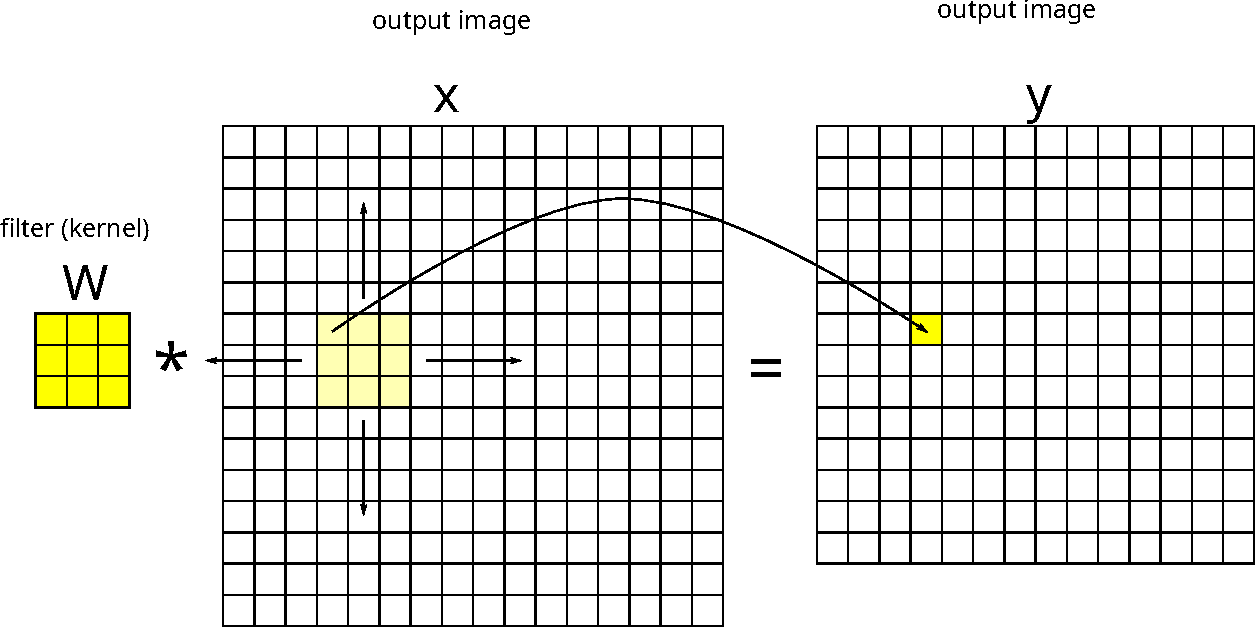
\includegraphics[width=0.8\textwidth]{out/pdf/svg/conv_1.pdf}
  \end{center}
\end{itemize}
\end{frame}

%%%%%%%%%%%%%%%%% 
\begin{frame}
  \frametitle{Convolution (a single channel version)}
\begin{itemize}
\item $W_{i,j}$ : a filter ($0 \leq i < K$, $0 \leq j < K$)
\item $b$ : bias
\item $x_{i,j}$ : an input image ($0 \leq i < H$, $0 \leq j < W$)
\item $y_{i,j}$ : an output image ($0 \leq i < H - K + 1$, $0 \leq j < W - K + 1$)
\end{itemize}
\begin{center}
  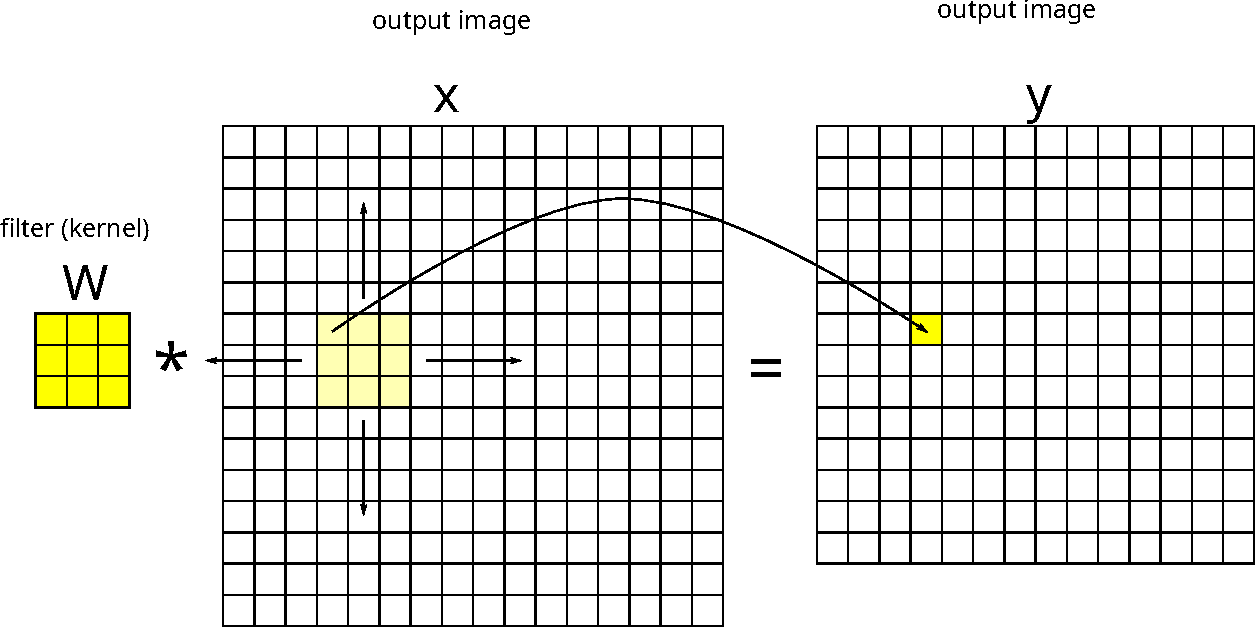
\includegraphics[width=0.5\textwidth]{out/pdf/svg/conv_1.pdf}
\end{center}

  \begin{eqnarray*}
\forall i, j \quad y_{i,j} & = & \sum_{0 \leq i' < K, 0 \leq j' < K} w_{i',j'} x_{i+i',j+j'} + b
  \end{eqnarray*}
  %           &  & \mbox{(for each $i,j$)}
\end{frame}


%%%%%%%%%%%%%%%%% 
\begin{frame}
  \frametitle{Convolution (multiple channels version)}
  \begin{itemize}
  \item say input has $IC$ channels and output $OC$ channels
  \item $W_{oc,ic,i,j}$ : filter ($0 \leq ic < IC$, $0 \leq oc < OC$)
  \item $b_{oc}$ : bias ($0 \leq oc < OC$)
  \item $x_{ic,i,j}$ : an input image
  \item $y_{oc,i,j}$ : an output image

    \begin{eqnarray*}
      \forall oc, i, j \quad
    y_{oc,i,j} & = & \sum_{ic,i',j'} w_{oc,ic,i',j'} x_{ic,i+i',j+j'} + b_{oc}\\
    \end{eqnarray*}

  \item the actual code does this for each sample in a batch
  \begin{eqnarray*}
    \forall s, oc, i, j \quad
    y_{s,oc,i,j} & = & \sum_{ic,i',j'} w_{oc,ic,i',j'} x_{s,ic,i+i',j+j'} + b_{oc}\\
  \end{eqnarray*}
\end{itemize}
\end{frame}

%%%%%%%%%%%%%%%%%
\begin{frame}
  \frametitle{Convolution (Back propagation 1)}
  \begin{itemize}
  \item $\pp{L}{x}$
    \begin{eqnarray*}
      \pp{L}{x_{s,ic,i+i',j+j'}}
      & = & \sum_{s',oc,i,j} \pp{L}{y_{s',oc,i,j}} \pp{y_{s',oc,i,j}}{x_{s,ic,i+i',j+j'}} \\
      & = & \sum_{oc,i,j} \pp{L}{y_{s,oc,i,j}} w_{oc,ic,i',j'} 
    \end{eqnarray*}
  \end{itemize}
\end{frame}

%%%%%%%%%%%%%%%%%
\begin{frame}
  \frametitle{Convolution (Back propagation 2)}
  \begin{itemize}
  \item $\pp{L}{w}$
    \begin{eqnarray*}
      \pp{L}{w_{oc,ic,i',j'}}
      & = & \sum_{s,oc',i,j} \pp{L}{y_{s,oc',i,j}} \pp{y_{s,oc',i,j}}{w_{oc,ic,i',j'}} \\
      & = & \sum_{s,i,j} \pp{L}{y_{s,oc,i,j}} x_{s,ic,i+i',j+j'}
    \end{eqnarray*}

  \item $\pp{L}{b}$
    \begin{eqnarray*}
      \pp{L}{b_{oc}}
      & = & \sum_{s,oc',i,j} \pp{L}{b_{oc}} \pp{y_{s,oc',i,j}}{b_{oc}} \\
      & = & \sum_{s,i,j} \pp{L}{y_{s,oc,i,j}}
    \end{eqnarray*}
  \end{itemize}
\end{frame}


%%%%%%%%%%%%%%%%%
\begin{frame}
\frametitle{Linear (a.k.a. Fully Connected Layer)}
\begin{itemize}
\item \ao{\textbf{definition:}}
\begin{eqnarray*}
  y = \mbox{Linear}(W; x) & \equiv & Wx + b \\
  \forall i \quad y_i & = & \sum_{j} W_{ij}x_j + b_i
\end{eqnarray*}
\end{itemize}
\end{frame}


%%%%%%%%%%%%%%%%% 
\begin{frame}
\frametitle{Linear (Back Propagation 1)}
\begin{itemize}
\item $\pp{L}{x}$
    \begin{eqnarray*}
      \pp{L}{x_j} 
      & = & \sum_{i'} \pp{L}{y_{i'}} \pp{y_{i'}}{x_j} \\
      & = & \sum_{i'} \pp{L}{y_{i'}} w_{i'j} \\
    \end{eqnarray*}
  \end{itemize}
\end{frame}

%%%%%%%%%%%%%%%%% 
\begin{frame}
\frametitle{Linear (Back Propagation 2)}
\begin{itemize}
\item $\pp{L}{W}$
  \begin{eqnarray*}
    \pp{L}{W_{ij}} 
    & = & \sum_{i'} \pp{L}{y_{i'}} \pp{y_{i'}}{W_{ij}} \\
    & = & \pp{L}{y_{i}} x_j
  \end{eqnarray*}
  
\item $\pp{L}{b}$
  \begin{eqnarray*}
    \pp{L}{b_i} 
    & = & \sum_{i'} \pp{L}{y_{i'}} \pp{y_{i'}}{b_i} \\
    & = & \pp{L}{y_{i}}
  \end{eqnarray*}
\end{itemize}
\end{frame}

%%%%%%%%%%%%%%%%% 
\begin{frame}
\frametitle{ReLU}
\begin{itemize}
\item \ao{\textbf{definition (scalar ReLU):}}
for $x \in R$, define
\begin{eqnarray*}
\relu(x) & \equiv & \max(x, 0) 
\end{eqnarray*}

\item \ao{\textbf{derivatives of relu:}} for $y = \relu(x)$, 
\[ \pp{y}{x} = \left\{
\begin{array}{ll}
1 & (x > 0) \\
0 & (x \leq 0)
\end{array}
\right. 
= \max(\sign(x), 0)
\]
\end{itemize}

\begin{center}
\def\svgwidth{0.6\textwidth}
\input{out/tex/svg/relu.pdf_tex}
\end{center}
\end{frame}


%%%%%%%%%%%%%%%%% 
\begin{frame}
\frametitle{ReLU}
\begin{itemize}
\item \ao{\textbf{definition (vector ReLU):}}
for a vector $x \in R^n$, define $\ReLU$ as the application
of $\relu$ to each component
\begin{eqnarray*}
\ReLU(x) & \equiv & \vecthree{\relu(x_0)}{\vdots}{\relu(x_{n-1})}
\end{eqnarray*}

\item \ao{\bf derivatives of ReLU:} 
  \begin{eqnarray*}
    \pp{y_j}{x_i} & = & \left\{
                        \begin{array}{ll}
                          \max(\sign(x_i), 0) & (i = j) \\
                          0 & (i \neq j) \\
                        \end{array}
                        \right.
  \end{eqnarray*}
\end{itemize}
\end{frame}

%%%%%%%%%%%%%%%%% 
\begin{frame}
\frametitle{ReLU}
\begin{itemize}
\item \ao{\textbf{back propagation:}}
  \begin{eqnarray*}
    \pp{L}{x_j} & = & \sum_i \pp{L}{y_i} \pp{y_i}{x_j} \\
                & = & \pp{L}{y_j} \pp{y_j}{x_j} \\
                & = & \left\{
                      \begin{array}{ll}
                        {\displaystyle \pp{L}{y_j}} & (x_j \geq 0) \\
                        0 & (x_j < 0) \\
                      \end{array}
    \right.
  \end{eqnarray*}
\end{itemize}
\end{frame}

  
\iffalse
%%%%%%%%%%%%%%%%% 
\begin{frame}
\frametitle{A remark on ReLU's derivative (1)}
\begin{itemize}
\item it is a diagonal matrix whose elements are either 1 or 0
\item if ReLU is combined with another scalar
  field (i.e. $z = f(y) = f(\ReLU(x))$), no points in 
  literally making the matrix and multiplying it
\item let us write ${\displaystyle \pp{z}{y} = (a_0\; \cdots\; a_{n-1})}$
{\footnotesize
\begin{eqnarray*}
 \pp{z}{x} 
& = & \pp{z}{y} \pp{y}{x} \\
& = & (a_0\; \cdots\; a_{n-1}) \mathree{\max(\sign(x_0, 0))}{\cdots}{0}
              {\vdots}{\ddots}{\vdots}
              {0}{\cdots}{\max(\sign(x_{n-1}, 0))} \\
& = & (a_0 \max(\sign(x_0, 0))\;\;\cdots\;\;a_{n-1} \max(\sign(x_{n-1}, 0))
\end{eqnarray*}}
\end{itemize}
\end{frame}


%%%%%%%%%%%%%%%%% 
\begin{frame}
\frametitle{A remark on ReLU's derivative (2)}
\begin{itemize}
\item if we define $\relutwo(a,x) = a * \max(\sign(x), 0)$
and $\ReLUtwo$ by its elementwise application, then it holds:
\begin{eqnarray*}
 \pp{z}{x} & = & \ReLUtwo\left(\pp{z}{y}, x\right)
\end{eqnarray*}
\item i.e., zero elements of ${\displaystyle\pp{z}{y}}$ for which
  the corresponding element of $x$ is negative
\end{itemize}
\end{frame}
\fi


%%%%%%%%%%%%%%%%% 
\begin{frame}
\frametitle{softmax}
\begin{itemize}
\item \ao{\textbf{definition:}} for $x \in R^n$
\begin{eqnarray*}
y = \softmax(x)
& \equiv & 
\frac{1}{\sum_{i=0}^{n-1} \exp(x_j)} \vecthree{\exp(x_0)}{\vdots}{\exp(x_{n-1})} \\
\end{eqnarray*}
it is a vector whose:
\begin{itemize}
\item each component $> 0$,
\item sum of all components $= 1$
\item largest component ``dominates''
\end{itemize}
\end{itemize}

\begin{center}
\def\svgwidth{0.65\textwidth}
{\large\input{out/tex/svg/softmax.pdf_tex}}
\end{center}
\end{frame}

%%%%%%%%%%%%%%%%% 
\begin{frame}
\frametitle{$\log\softmax$}
\begin{itemize}
\item []
  \begin{eqnarray*}
y & = & \log(\softmax(x)) \\
  & = & 
\vecthree{x_0 - \log\sum_{i=0}^{n-1}\exp(x_i)}{\vdots}{x_{n-1} - \log\sum_{i=0}^{n-1}\exp(x_i)}
\end{eqnarray*}

\item (recall
\begin{eqnarray*}
\softmax(x)
& \equiv & 
\frac{1}{\sum_{i=0}^{n-1} \exp(x_j)} \vecthree{\exp(x_0)}{\vdots}{\exp(x_{n-1})} \\
\end{eqnarray*})

\end{itemize}

\end{frame}

%%%%%%%%%%%%%%%%% 
\begin{frame}
  \frametitle{$\nll$}
  \begin{itemize}
  \item \ao{\textbf{definition:}}
    \begin{itemize}
    \item $x$ : $n$-vector
      % whose $x_i$ is the predicted probability that
      % data belongs to class $i$
    \item $t$ : true class of the data
    \end{itemize}
    \begin{eqnarray*}
      \nll(x, t)  & \equiv & -\log x_t
    \end{eqnarray*}
  \item thus,
    \begin{eqnarray*}
      y & = & \nll (\softmax (x), t) \\
        & = & -x_t + \log\sum_{i=0}^{n-1}\exp(x_i)
    \end{eqnarray*}
  \end{itemize}
\end{frame}


%%%%%%%%%%%%%%%%% 
\begin{frame}
  \frametitle{$\nll\; \softmax$ (Back propagation)}
  \begin{itemize}
  \item 
\begin{eqnarray*}
  \pp{L}{x_i} & = & \pp{L}{y} \pp{y}{x_i} \\
              & = & \left\{\begin{array}{ll}
                             \pp{L}{y} (-1 + \frac{\exp(x_i)}{\sum_{i=0}^{n-1}\exp(x_i)}) & (i = t) \\
                             \pp{L}{y} \frac{\exp(x_i)}{\sum_{i=0}^{n-1}\exp(x_i)} & (i \neq t)
                          \end{array}\right. \\
              & = & \left\{\begin{array}{ll}
                            \pp{L}{y} \; (-1 + \softmax(x_i)) & (i = t) \\
                            \pp{L}{y} \; \softmax(x_i) & (i \neq t)
                          \end{array}\right.
\end{eqnarray*}
  \end{itemize}
\end{frame}

%%%%%%%%%%%%%%%%% 
\begin{frame}
\frametitle{Note: why $\nll\; \softmax$?}
\begin{itemize}
\item recall that for $n$-way classification,
  the output of $p = \softmax(\ldots)$ is an $n$-vector 
\item $p_i$ is meant to be the {\it probability} that
  a particular sample belongs to the class $i$
\item for that purpose, a loss function could be
  any function that decreases with $p_t$
  (something as simple as $- p_t$),
  where $t$ is the true label of the particular sample
\item we isntead use $\nll(p, t) = -\log p_t$. why?
\end{itemize}
\end{frame}

%%%%%%%%%%%%%%%%% 
\begin{frame}
\frametitle{Note: why $\nll\log\softmax$?}
\begin{itemize}
\item this is because,
  \begin{enumerate}
  \item the goal is to maximize
    the joint probability of the entire data, which is
    the {\it product} of probabilities of individual samples:
    \[ \Pi_k p_{t_k}, \]
    where $t_k$ is the true label of sample $k$, and
  \item the loss over a mini-batch is
    the {\it sum} of losses of individual samples
  \end{enumerate}
\item they can be reconciled by setting the loss function
  to $-\log p_t$
  \[ \sum_k \left(-\log p_{t_k}\right) = - \log\left(\Pi_k p_{t_k}\right) \]
\end{itemize}
\end{frame}

\end{document}


%%%%%%%%%%%%%%%%% 
\begin{frame}
\frametitle{Derivative of softmax}
\begin{itemize}
\item for $y = \softmax(x)$, ${\displaystyle\left(\pp{y}{x}\right)}$
is an $n\times n$ matrix whose elements are given by:
\begin{itemize}
\item (diagonal elements)
  \begin{eqnarray*}
\left(\pp{y}{x}\right)_{i,i} 
& = & \pp{}{x_i} \frac{\exp(x_i)}{\sum_k \exp(x_k)} \\
& = & \frac{\exp(x_i)\sum_k\exp(x_k) - \exp(x_i)^2}{\left(\sum_k \exp(x_k)\right)^2} \\
& = & \ao{y_i (1 - y_i)}
  \end{eqnarray*}
\item (non-diagonal elements) for $i \neq j$,
  \begin{eqnarray*}
\left(\pp{y}{x}\right)_{i,j} 
& = & \pp{}{x_j} \frac{\exp(x_i)}{\sum_k \exp(x_k)} \\
& = & - \exp(x_i) \frac{\exp(x_j)}{\left(\sum_k \exp(x_k)\right)^2} \\
& = & \ao{- y_i y_j}
  \end{eqnarray*}
\end{itemize}
\end{itemize}
\end{frame}


%%%%%%%%%%%%%%%%% 
\begin{frame}
\frametitle{Cross entropy}
\begin{itemize}
\item \ao{\textbf{definition:}} for $y \in R^n$,
\begin{eqnarray*}
H(t, y) & \equiv & - \sum_{i=0}^{n-1} t_i \log y_i
\end{eqnarray*}
\item \ao{\textbf{derivative of $H$:}} 
for $z = H(t, y)$, ${\displaystyle \pp{z}{y}}$ is an $n$-vector
\begin{eqnarray*}
\pp{z}{y} 
& = & - \left(\frac{t_0}{y_0}\; \cdots \; \frac{t_{n-1}}{y_{n-1}}\right) \\
\end{eqnarray*}
\item if $t$ is a one hot vector, so is this vector; if $t = \textbf{c}$, 
\begin{eqnarray*}
\pp{z}{y} 
& = & - \left(0\;\cdots\;0\;\frac{1}{y_c}\;0\;\cdots\;0\right) \\
& = & \ao{- \frac{\textbf{c}}{y_c}}
\end{eqnarray*}
\end{itemize}
\end{frame}

%%%%%%%%%%%%%%%%% 
\begin{frame}
\frametitle{Composition of softmax and cross entropy}
\begin{itemize}
\item [] In particular, composition of softmax and $H$ enjoy a remarkable simplification when differentiated:
\begin{itemize}
\item for $z = H(t,y) = H(t, \softmax(x))$, 
\begin{eqnarray*}
\pp{z}{x} 
& = & \pp{z}{y} \pp{y}{x} \\
& = & - \frac{\textbf{c}}{y_c} \pp{y}{x}  \\
& = & - \frac{1}{y_c} \pp{y_c}{x}  \\
& = & \frac{1}{y_c} 
(y_0y_c\;\;y_1y_c\;\;\cdots\;\;y_c(1-y_c)\;\;y_{c+1}y_c\;\;\cdots\;\;y_{n-1}y_c)  \\
& = & (y_0\;\;y_1\;\;\cdots\;\;(y_c-1)\;\;y_{c+1}\;\;\cdots\;\;y_{n-1}) \\
& = & \ao{{}^t(y - t)} \\
\end{eqnarray*}
\end{itemize}
\end{itemize}
\end{frame}

\end{document}


%%%%%%%%%%%%%%%%% 
\section{Putting them together}
%%%%%%%%%%%%%%%%% 

%%%%%%%%%%%%%%%%% 
\subsection{Column vectors version}
%%%%%%%%%%%%%%%%% 

%%%%%%%%%%%%%%%%% 
\begin{frame}
\begin{columns}
\begin{column}{0.45\textwidth}
\begin{itemize}
\item put them together
\item $x, x_1, \cdots, x_5, y$ are \ao{column} vectors
\item ${\displaystyle\pp{e}{x_i}}$ are \ao{row} vectors
\end{itemize}

{\small
\begin{eqnarray*}
x_1 & = & W_0x \\
x_2 & = & \ReLU(x_1) \\
x_3 & = & W_1x_2 \\
x_4 & = & \ReLU(x_3) \\
x_5 & = & W_2x_4 \\
  y & = & \softmax(x_5) \\
  e & = & H(t, y)
\end{eqnarray*}}
\end{column}

\begin{column}{0.55\textwidth}
{\small
\begin{eqnarray*}
\pp{e}{x_5} & = & {}^t(y - t) \\
\pp{e}{x_4} & = & \pp{e}{x_5} W_2 \\
\pp{e}{x_3} & = & \ReLUtwo(\pp{e}{x_4}, x_3) \\
\pp{e}{x_2} & = & \pp{e}{x_3}W_1 \\
\pp{e}{x_1} & = & \ReLUtwo(\pp{e}{x_2}, x_1) \\
 & & \\
\pp{e}{W_2} & = & {}^t \pp{e}{x_5} \; {}^tx_4 \\
\pp{e}{W_1} & = & {}^t \pp{e}{x_3} \; {}^tx_2 \\
\pp{e}{W_0} & = & {}^t \pp{e}{x_1} \; {}^tx 
\end{eqnarray*}}
\end{column}
\end{columns}
\end{frame}

%%%%%%%%%%%%%%%%% 
\subsection{Row vectors version}
%%%%%%%%%%%%%%%%% 

%%%%%%%%%%%%%%%%% 
\begin{frame}
\frametitle{``Row vectors'' version}
\begin{itemize}
\item it is often more convenient to think vectors 
  $x, x_1, \cdots , x_{n-1}, y$ as \ao{\emph{row}} vectors
\item matrices are multiplied from right, not left
\item derivatives become \ao{\emph{column}} vectors
\[ f(x + \Delta x) \approx f(x) + \ao{\Delta x f'(x)} \]
\item the righthand side of the chain rule flips
\[ \pp{z}{x} = \pp{y}{x} \pp{z}{y} \]
\item the chain rule for matrix also slightly changes. for
a scalar $z$:
\[ z = f(y) = f(x w) \]
\begin{eqnarray*}
\pp{z}{w} & = & {}^tx \; {}^t\pp{z}{y}
\end{eqnarray*}
\end{itemize}
\end{frame}


%%%%%%%%%%%%%%%%% 
\begin{frame}
\frametitle{``Column vector'' vs. ``Row vector''}

\begin{tabular}{|l|c|c|}\hline
                       & column version & row version \\\hline
$x, x_i, \cdots$       & column         & row         \\
${\displaystyle \pp{e}{x_i}} \cdots$   & row            & column      \\
& & \\
chain rule             & ${\displaystyle \pp{z}{x} = \pp{z}{y} \pp{y}{x}}$
                       & ${\displaystyle \pp{z}{x} = \pp{y}{x} \pp{z}{y}}$ \\
& & \\
chain rule 
                       & ${\displaystyle \pp{z}{w} = {}^t\pp{z}{y} {}^tx}$
                       & ${\displaystyle \pp{z}{w} = {}^tx \; {}^t\pp{z}{y}}$ \\
for $z = f(y) = f(wx)$ or $f(xw)$ & & \\\hline
\end{tabular}
\end{frame}

%%%%%%%%%%%%%%%%% 
\begin{frame}
\frametitle{}

\begin{columns}
\begin{column}{0.5\textwidth}
\begin{itemize}
\item \ao{``row vectors''} version:
\item $x, x_1, \cdots, x_5, y$ are \ao{row} vectors
\item ${\displaystyle\pp{e}{x_i}}$ are \ao{column} vectors
\end{itemize}
{\small
\begin{eqnarray*}
x_1 & = & \ao{x W_0} \\
x_2 & = & \ReLU(x_1) \\
x_3 & = & \ao{x_2 W_1} \\
x_4 & = & \ReLU(x_3) \\
x_5 & = & \ao{x_4 W_2} \\
  y & = & \softmax(x_5) \\
  e & = & H(t, y)
\end{eqnarray*}}
\end{column}

\begin{column}{0.5\textwidth}
{\small
\begin{eqnarray*}
\pp{e}{x_5} & = & {}^t (y - t) \\
\pp{e}{x_4} & = & \ao{W_2 \pp{e}{x_5}} \\
\pp{e}{x_3} & = & \ReLUtwo(\pp{e}{x_4}, x_3) \\
\pp{e}{x_2} & = & \ao{W_1 \pp{e}{x_3}} \\
\pp{e}{x_1} & = & \ReLUtwo(\pp{e}{x_2}, x_1) \\
 & & \\
\pp{e}{W_2} & = & \ao{{}^t x_4 \; {}^t \pp{e}{x_5}} \\
\pp{e}{W_1} & = & \ao{{}^t x_2 \; {}^t \pp{e}{x_3}} \\
\pp{e}{W_0} & = & \ao{{}^t x   \; \pp{e}{x_1}}
\end{eqnarray*}}
\end{column}
\end{columns}
\end{frame}


%%%%%%%%%%%%%%%%% 
\subsection{All row vectors version}
%%%%%%%%%%%%%%%%% 

%%%%%%%%%%%%%%%%% 
\begin{frame}
\frametitle{Make everything row vectors}
\begin{itemize}
\item finally, it's more convenient to compute ${\displaystyle {}^t \pp{e}{x_i}}$
instead of ${\displaystyle \pp{e}{x_i}}$, to make all vectors row vectors
\end{itemize}
\end{frame}

%%%%%%%%%%%%%%%%% 
\begin{frame}
\frametitle{}
\begin{columns}
\begin{column}{0.5\textwidth}
\begin{itemize}
\item \ao{``all row vectors''} version:
\item $x, x_1, \cdots, x_5, y$ are \ao{row} vectors
\item compute ${\displaystyle {}^t\pp{e}{x_i}}$ 
  (\ao{row} vectors) instead of ${\displaystyle \pp{e}{x_i}}$
\end{itemize}
{\small
\begin{eqnarray*}
x_1 & = & x W_0 \\
x_2 & = & \ReLU(x_1) \\
x_3 & = & x_2 W_1 \\
x_4 & = & \ReLU(x_3) \\
x_5 & = & x_4 W_2 \\
  y & = & \softmax(x_5) \\
  e & = & H(t, y)
\end{eqnarray*}}
\end{column}

\begin{column}{0.5\textwidth}
{\small
\begin{eqnarray*}
{}^t \pp{e}{x_5} & = & y - t \\
{}^t \pp{e}{x_4} & = & {}^t \pp{e}{x_5}\; {}^tW_2  \\
{}^t \pp{e}{x_3} & = & {}^t \ReLUtwo(\pp{e}{x_4}, x_3) \\
{}^t \pp{e}{x_2} & = & {}^t \pp{e}{x_3} \; {}^tW_1 \\
{}^t \pp{e}{x_1} & = & {}^t \ReLUtwo(\pp{e}{x_2}, x_1) \\
 & & \\
\pp{e}{W_2} & = & {}^t x_4 \; {}^t \pp{e}{x_5} \\
\pp{e}{W_1} & = & {}^t x_2 \; {}^t \pp{e}{x_3} \\
\pp{e}{W_0} & = & {}^t x   \; {}^t \pp{e}{x_1}
\end{eqnarray*}}
\end{column}
\end{columns}
\end{frame}

%%%%%%%%%%%%%%%%% 
\begin{frame}
\frametitle{mini batch}

\begin{itemize}
\item the code is implementing the ``all rows'' version
\item each iteration processes a number of samples (mini batch)
\item each vector now becomes a matrix, stacking samples (row vectors) vertically
\end{itemize}

\end{frame}



\end{document}





%%%%%%%%%%%%%%%%% 
\begin{frame}
  \frametitle{Chain Rule}

  \[ \left(x_i\right)_{0\leq i \leq m} \rightarrow
    \left(y_j\right)_{0\leq j \leq n} \rightarrow L \]
  
  \[ \frac{\partial L}{\partial x_i}
    = \sum_j \frac{\partial L}{\partial y_j}
    \frac{\partial y_j}{\partial x_i}  \]
  
\end{frame}

%%%%%%%%%%%%%%%%% 
\begin{frame}
\frametitle{Convolution2D}
\[ H = (K - 1) / 2 \]
  
\[ y(b,oc,i,j) = \sum_{{\scriptsize
      \begin{array}{c}
        0\leq ic\leq IC, \\
        -H\leq i'\leq H, \\
        -H\leq j'\leq H
      \end{array}}}
  w(oc,ic,H+i',H+j') \, x(b,ic,i+i',j+j')
\]

\[ y(b,oc,i,j) = \sum_{{\scriptsize
      \begin{array}{c}
        0\leq ic\leq IC, \\
        -H+i\leq i'\leq H+i, \\
        -H+j\leq j'\leq H+j
      \end{array}}}
  w(oc,ic,H+i'-i,H+j'-j) \, x(b,ic,i',j')
\]

\[
  \frac{y(b,oc,i,j)}{x(b,ic,i',j')} = w(oc,ic,H+i'-i,H+j'-j)
\]

\begin{eqnarray*}
  &   & \frac{L}{x(b,ic,i',j')} \\
  & = & \sum_{b,oc,i,j} \frac{L}{y(b,oc,i,j)} \frac{y(b,oc,i,j)}{x(b,ic,i',j')} \\
  & = & \sum_{b,oc,i,j} \frac{L}{y(b,oc,i,j)} w(oc,ic,H+i'-i,H+j'-j)
\end{eqnarray*}

\end{frame}
\end{document}


